\chapter{FL architecture \& design} %spasimo se fl architecture
\label{Chapter-FL-architecture-design}

%%%%%%%%%%%%%%%%%%%%%%%%%%%%%%%%%%%%%%%%%%%%%%%%%%%%% Software %%%%%%%%%%%%%%%%%%%%%%%%%%%%%%%%%%%%%%%%%%%%%%%%%%%%% 
\section{Software}
\subsection{Tensorflow \& Keras}
TensorFlow \cite{tensorflow2015-whitepaper} is an interface for expressing ML algorithms and an implementation for executing such algorithms. It offers a complete, flexible ecosystem of tools, libraries and community resources that that facilitates the development and deployment of ML powered applications. Its main advantage is the ability to use high-level APIs like Keras with eager execution, enabling immediate model iteration and easy debugging. 

Tesnorflow \& Keras were used in all experiments during modelization. It is chosen due to its simple, flexible architecture, which turns new ideas into code quickly. In addition, due to the existence of TensorFlow Federated (TFF) \cite{tff} framework, there are many compatible theoretical resources and tutorials. TFF is simulating FL to facilitate research and experimentation with FL algorithms, thus it is incompatible with this work which aims to implement real-world FL with hardware accelerators.

\subsection{Python/C API} \label{Python/C API}
As the goal is to integrate FL with FPGA accelerators, the majority of the codebase is developed in C++. This include all the networking, communication, model aggregation and any required model transformations. TensorFlow on Python is utilized for model evaluation and, throughout the modelization phase, for training. To connect these two components, the Python interpreter is embedded to the core program using the Python/C API \cite{Python/C_API, embedding_python}.

With the TensorFlow C API \cite{TF_C_API}, TensorFlow could be used directly in C++, however several capabilities, like the Neural Network library, are not supported. Furthermore, quickly rotating among ANN architectures, training techniques, etc. is quite usual in FL development. With the C API that becomes tedious and slow, since it is geared more toward uniformity and simplicity than convenience, and C++ needs to be recompiled after every change. Due to these factors, integrating the Python interpreter and using TensorFlow in Python is considered as a more appropriate solution.

\subsection{POSIX sockets}
POSIX sockets \cite{POSIX_socket} is an application programming interface (API) for Internet and Unix domain sockets, used for inter-process communication (IPC). A socket is an abstract representation for the local endpoint of a network communication path. According to the Unix philosophy, the POSIX sockets API defines it as a file descriptor that offers a standard interface for input and output to data streams.

The 4.2 Berkeley Software Distribution \cite{bsd} Unix operating system, which was introduced in 1983, is where the API originates from. POSIX sockets transitioned mostly unchanged from a de facto standard to a POSIX specification component. They are commonly referred to as "Berkeley sockets" or "BSD sockets" to acknowledge the Berkeley Software Distribution, where they were first implemented.
 
In FL, entities possess their own private data. This is best implemented through processes with private data space that communicate using sockets. Therefore, the POSIX socket API implementation provided by the LINUX operating system is used for all inter-entity communication. 

POSIX sockets can be configured for blocking or non-blocking operation. In blocking operation, the program halts until the entire message is sent or received. In contrast, during non-blocking operation they only retrieve or send data that is immediately available. Thus, the program does not stall on straggler connections and many deadlock situations are avoided, but there is no guarantees that the messages will be send or received in one piece, especially when said messages are large \footnote{This is due to limited sized socket buffers set up by the operating systems.}.

%%%%%%%%%%%%%%%%%%%%%%%%%%%%%%%%%%%%%%%%%%%%%%%%%%%%% Data Preparation %%%%%%%%%%%%%%%%%%%%%%%%%%%%%%%%%%%%%%%%%%%%%%%%%%%%% 
\section{Data Preparation}
\subsection{Normalization}
Dataset normalization \cite{dataset_norm}, as part of data preparation, is a standard practice in ML. Normalization transforms the features of a dataset to a common scale, without distorting discrepancies in the ranges of values or losing information. This technique prevents large scaled characteristics to dominate during training. Furthermore, many algorithms, such as ReLU non-linearities, exhibit better performance when fed with data of floating-point format.

In this work, the Fashion-MNIST dataset provided by TensorFlow Datasets \cite{TFDS} collection is utilized. It is consisted of gray-scale images, where each pixel is represented by an integer in the range \([0,255]\). They are normalized to floating-point format in the range \([0,1]\) with the script \texttt{prepare\_dataset.py}. Furthermore, to avoid repeating this procedure for every experiment, the processed dataset is saved on disk.

\subsection{Distribution}
In FL, each client is meant to have their own unique, individualized dataset. Given that the provided Fashion-MNIST dataset is a single, concentrated collection, it must be distributed among the clients in order for federated training to be possible. Two approaches of partitioning the data among the clients are explored:

\subsubsection{IID}
The data are randomly partitioned in equally sized shards, one for every client. For example, if there are 10 clients, each will receive a shard containing 6000 examples. Although this distribution is not IID in the strictest sense\footnote{Due the shards being mutually exclusive, knowing that an example belongs to one of them indicates that it does not exist in others shards. Thus, knowledge about the other local datasets can be inferred and independence is violated.}, it is closer to a real-world scenario and many issues, such as class underrepresentation, can be easily avoided.

\subsubsection{non-IID}
Although statistical challenges are not the focus of this study, some testing with non-IID data has been done for sake of completeness. The dataset is broken up into shards, each of which includes examples from only one label. Each client receives two shards of different labels. If there are 10 clients, for instance, twenty shards will be produced, and each client will receive 3000 examples from two labels for a total of 6000 examples. Despite such a pathological non-IID distribution being atypical of a real-world scenario, it will assist investigate how severely the algorithms fail on extremely non-IID data.

\subsection{Pipeline}
The input pipeline that feeds the training data to the models is constructed using the \texttt{tf.data} API provided by TensorFlow. More specifically, before training begins, each client optimizes the use of its dataset by transforming it through caching, shuffling, batching, prefetching, and repeating. Additionally, this process is parameterized for flexibility and enable experimentation with different local dataset and batch sizes.

%%%%%%%%%%%%%%%%%%%%%%%%%%%%%%%%%%%%%%%%%%%%%%%%%%%%% Embedding Python Interpreter %%%%%%%%%%%%%%%%%%%%%%%%%%%%%%%%%%%%%%%%%%%%%%%%%%%%%
\section{Embedding the Python Interpreter}
As mentioned in section \ref{Python/C API}, the Python Interpreter is embedded on top of the C++ codebase. To make this integration as seamless as possible from both sides, an integration layer that operates as a wrapper for the C/Python API, has been developed. The C++ codebase can call Python code with simple function calls, while the Python code can access data from the C++ space like it would access data from its own space.

To achieve this, A number of steps need to be completed. First of all, a strait-forward abstract class is defined, which specifies a train and an evaluate function, as well as an input and an output model. The C++ codebase is interfacing with an implementation of this class. Its tasks include initializing the Python interpreter, loading the appropriate Python module, passing the necessary data and creating C++ function wrappers for the Python function.

Moving data from one side to the other can be trickier than it first appears. Using the appropriate API calls, such as \texttt{PyModule\_AddIntConstant}, simple constants and macros can be passed by copy to the Python module in a strait-forward manner. This approach fails when dealing with large amounts of data, such as the model parameters. Instead, by constructing NumPy array metadata over them and copying them, they can be passed by reference. In this manner, both ends observe the same memory space and there is no significant data copy.

After exposing the parameters to the Python code, one more step is necessary to enable the TesnorFlow library to be able to use them. In order to assign the received parameters to the model under training, they must be first transformed into TesnorFlow tensors with dimensions and shapes that match its layers. Likewise, to extract parameters from a model and expose them to the C++ codebase, its layers must be concated in a NumPy array.


\begin{figure}[H]
    \centering
        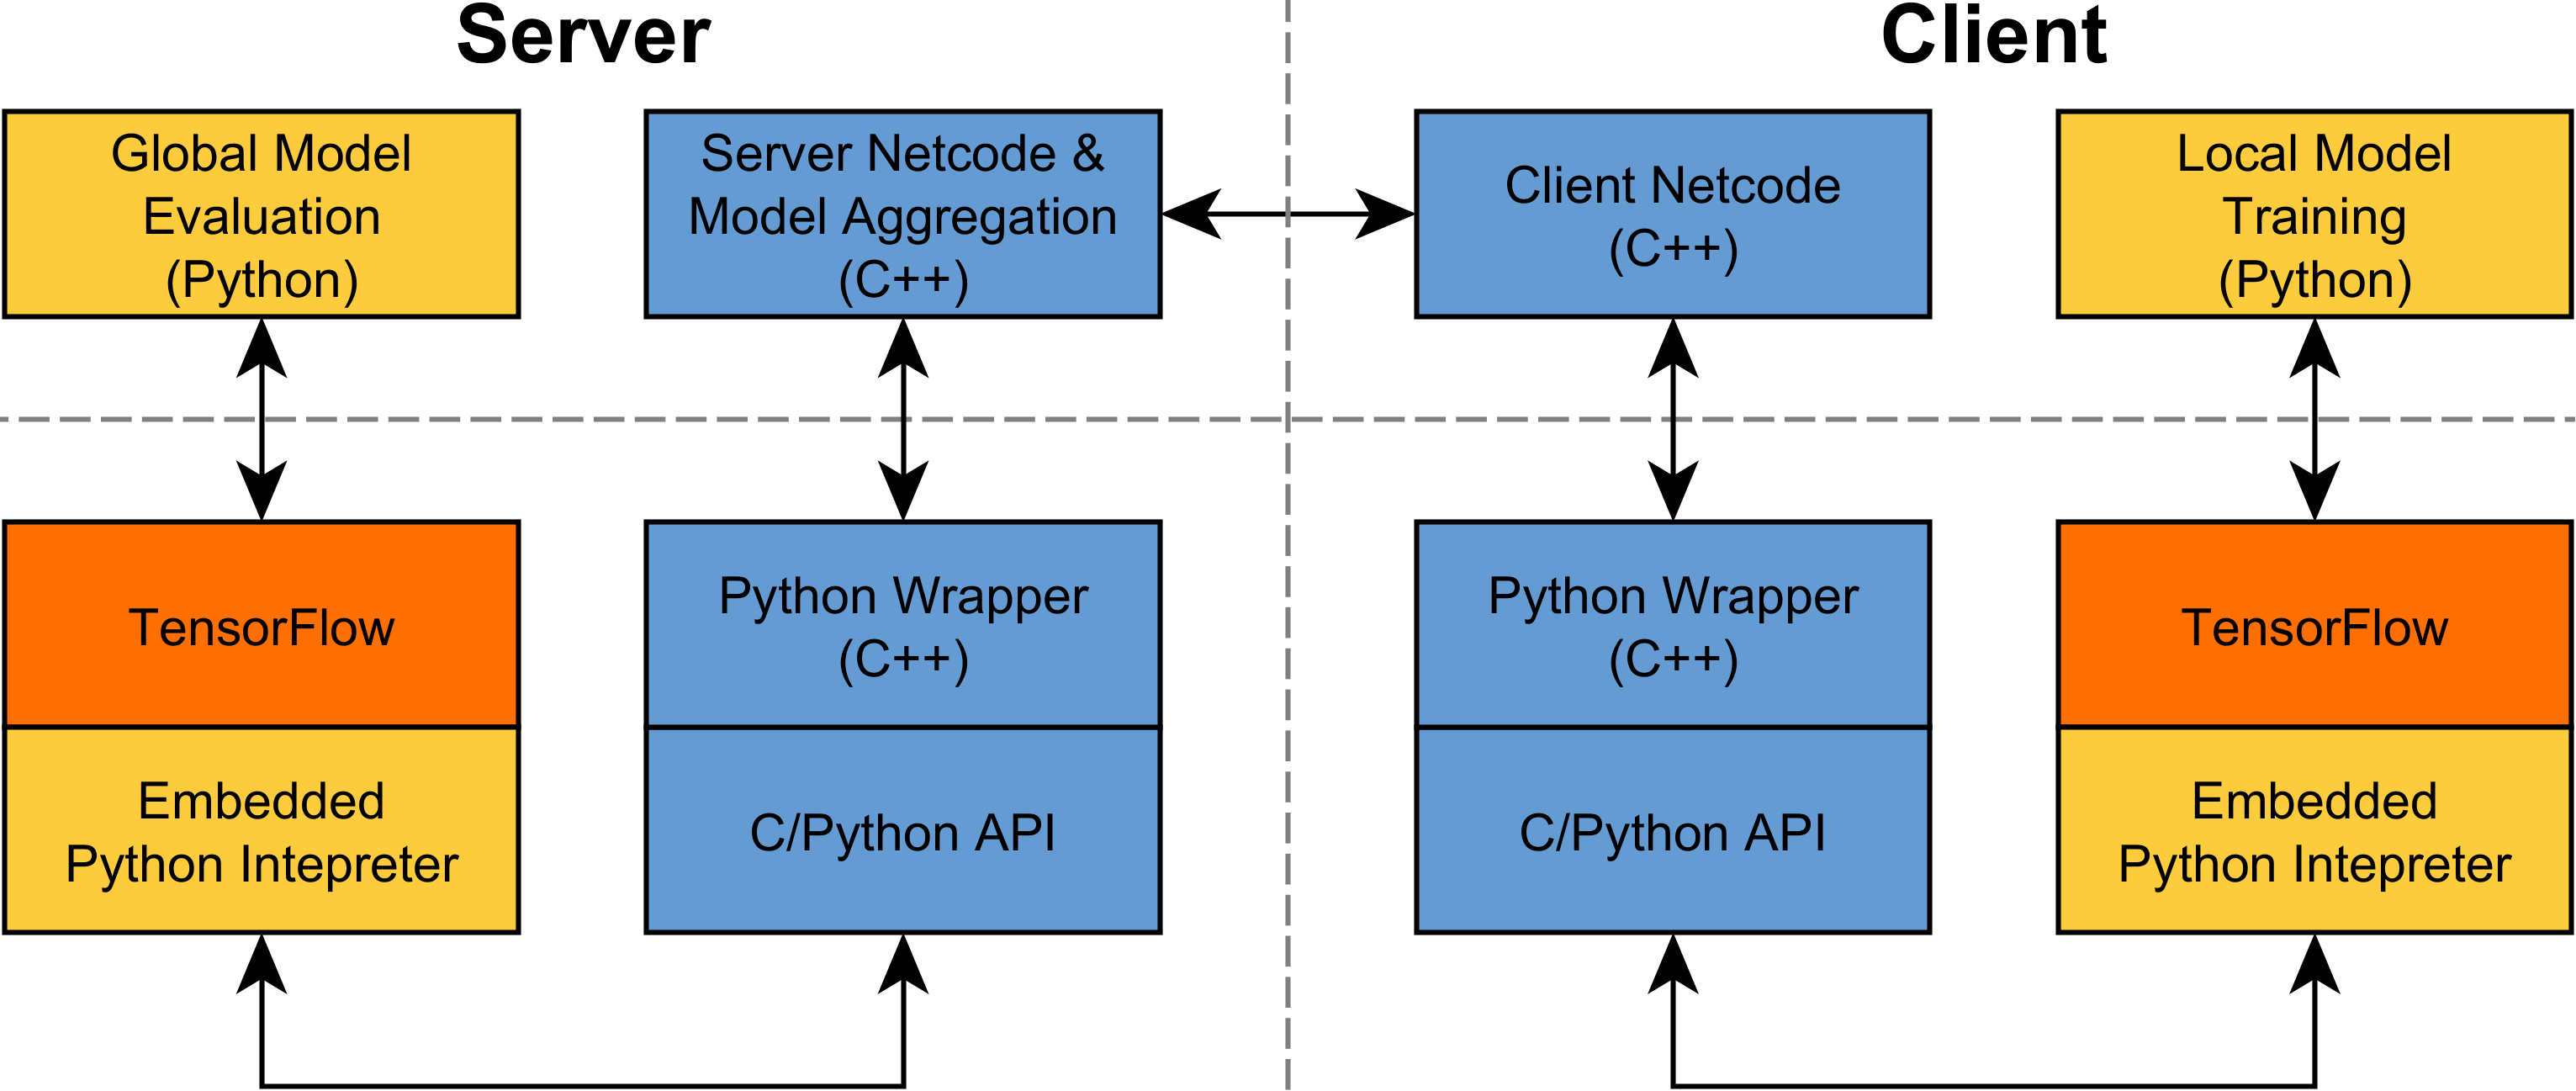
\includegraphics[width=1\textwidth]{Images/block_diagrams/model_lifecycle.png}
        \decoRule
        \caption[C++/Python Integration]{Overview of the C++/Python Integration. The FL protocol implementation components are represented in the top half, while the required libraries, APIs, and wrappers are shown in the bottom half.}
        \label{fig:model_lifecycle}
\end{figure}

%%%%%%%%%%%%%%%%%%%%%%%%%%%%%%%%%%%%%%%%%%%%%%%%%%%%% implementation %%%%%%%%%%%%%%%%%%%%%%%%%%%%%%%%%%%%%%%%%%%%%%%%%%%%% 
\section{FL Architecture}\label{sec:FL_architecture}
The architecture aims to offer a generalized FL loop that enables the implementation of various FL algorithms. To achieve this, it is designed to be flexible and modular, with each FL operation, such as client selection and aggregation, having its own specialized function. Additionally, all relevant training parameters and hyper-parameters, such as local epochs or participating clients per epoch, are compiled in the \texttt{definitions.hpp} file. Since the entire codebase accesses them from there, testing and experimentation are streamlined and less prone to mistakes.

In FL, multiple entities are present, the orchestrating server and the clients training the global model. As the aim of this work is to implement FL with clients operating on separate devices, it is essential that each entity is a distinct process with its own private data-space. That data-space contains its private training or testing dataset, as well as its local or global models. All required communication is facilitated through POSIX sockets.

\begin{figure}[H]
    \centering
        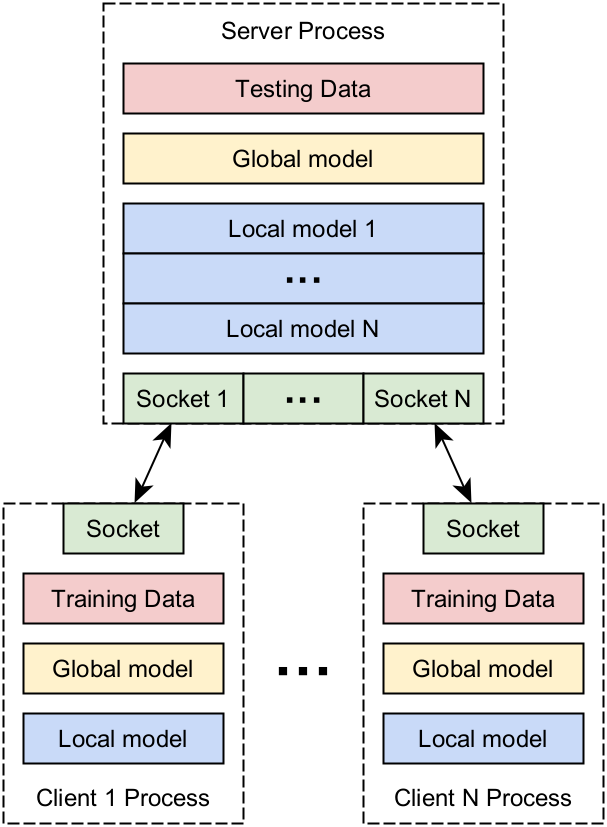
\includegraphics[width=0.5\textwidth]{Images/block_diagrams/memory_layout.png}
        \decoRule
        \caption[Process \& Memory layout]{Process and memory layout of the FL architecture. Each client holds their private data, the global model and the models they produced. Meanwhile, the server holds the testing dataset, the global model and the most recent local model it received. All communication goes through dedicated sockets.}
        \label{fig:process_mem_layout}
\end{figure}

\subsection{Server}
\subsubsection{Overview}
The server generally adheres to the event-driven server paradigm. The process, while sleeping, listens for events such as new connections or messages from the clients, and reacts according to their context. This is very similar to FL in that the server receives local models, aggregates them, and then, after accumulating a sufficient number of them, creates a new global model and announces it to the clients. All these actions are triggered by client updates.

The server process is the focal point of FL and is responsible for several tasks, which can be distinguished between algorithmic, systemic and auxiliary. Algorithmic tasks are the components of the FL algorithm, such as model aggregation. Systemic tasks are necessary operations to implement the FL algorithm, such as connecting sockets. In addition, some tasks that are not required to implement the algorithm are included in order to enhance its utility and ease development.

\subsubsection{Operation}
The server's first action is to load a pre-trained model, if one exists. While not a prerequisite to facilitate FL, this is done to enable transfer learning and experimenting with retraining a model under different settings. 

After that, the server completes a series of initializations. First of all, a listening socket is set-up in non-blocking operation, and the event-driven structure is established. Furthermore, the Python environment, where the global models are evaluated, is embedded and initialized. Finally, any structures or variables required by the FL algorithm are initialized.

After the initializations, the server enters a waiting state. To achieve this the \texttt{poll(2)} system call, which puts the process to sleep until an event occurs, is used. Four types of events may happen:
\begin{itemize}[leftmargin=*]
    \item The listening socket encounters a new connection, meaning a new client requests to join in the federated training. The socket is cloned, the clone establish the connection with the client, and any necessary data structures are created.
    \item A connected socket encounters an error, such as an sudden disconnection. Unreliable clients are expected to continue being unreliable, thus the most prudent course of action is discarding them.
    \item A connected socket receives new data. As a message can consist of millions of weights, it may be received across multiple events and a collection mechanism is needed to fully retrieve it. To achieve this, it is necessary to track the size of the received data per client and ensure that there is always adequate memory available to store a message from each connected client. If the message is complete and valid, its local model is aggregated to next global model, and the related client is considered as non-working.
    \item A connected socket can send new data. This indicates that a socket designated to send the global model to its connected client, is available to do so. As mentioned before, the messages can be quite large, thus multiple events may be required to fully send them. To achieve this, tracking of the amount of transmitted data per connection is necessary. When a message is fully send, the related client is considered as working. Furthermore, as there no more data to send, the \texttt{POLLOUT} flag of the socket is disabled.
\end{itemize}

Following any event, the server determines whether a new epoch should begin. It takes in consideration how many local models were successfully received this epoch, how many clients are connected, and how many clients are still working. If the current epoch requires further work, the process returns to the waiting state and sleeps until a new event occurs.

If the contrary is true, the new global model is created by dividing the aggregated local models by the number of received local models during the current epoch. This new model is evaluated, and then shared with clients that where randomly selected using the Durstenfeld-Fisher-Yates shuffle algorithm \cite{Durstenfeld_Fisher_Yates_paper, Fisher_Yates_shuffle_wiki}. The only action needed to share the model with a client is enabling the \texttt{POLLOUT} flag of the corresponding socket; the event loop will handle sending the message.

The event loop's final step is to determine whether any further training is required. If the target accuracy is achieved or a predetermined number of GEs have been completed, the server shows any relevant statistics, stores the final global model to disk, and shuts down.

% \subsubsection{Memory layout}

\subsection{Client}
\subsubsection{Overview}
During an epoch, a participating client receives a global model, goes through a few local training rounds, and then sends the updated local model back to the server. Training cannot begin until the global model is fully received. Furthermore, after sending the local model, nothing further needs to be done until a new global model is received.

As a result, the client is controlled by its communication with the server, and a master-slave relationship is formed between them. To effectively implement this, client-side communication is blocking, meaning a client can not take any action until it has fully received or send its messages.

\subsubsection{Operation}
At startup, the client creates a socket and connects to the server. Additionally, it embeds and initializes the Python environment that is used for training.  Following these initializations, the process moves into its main loop.

The main loop contains three major operation. First, it receives the global model shared by the server. Then, it is trained with the local private data, creating a new local model. Finally, any required transformations, such as quantization and compression, are applied to the new model, which is then send to the server. This process is repeated until the server informs that there will be no more training with that client.

% \subsubsection{Memory layout}
\begin{figure}[H]
    \centering
        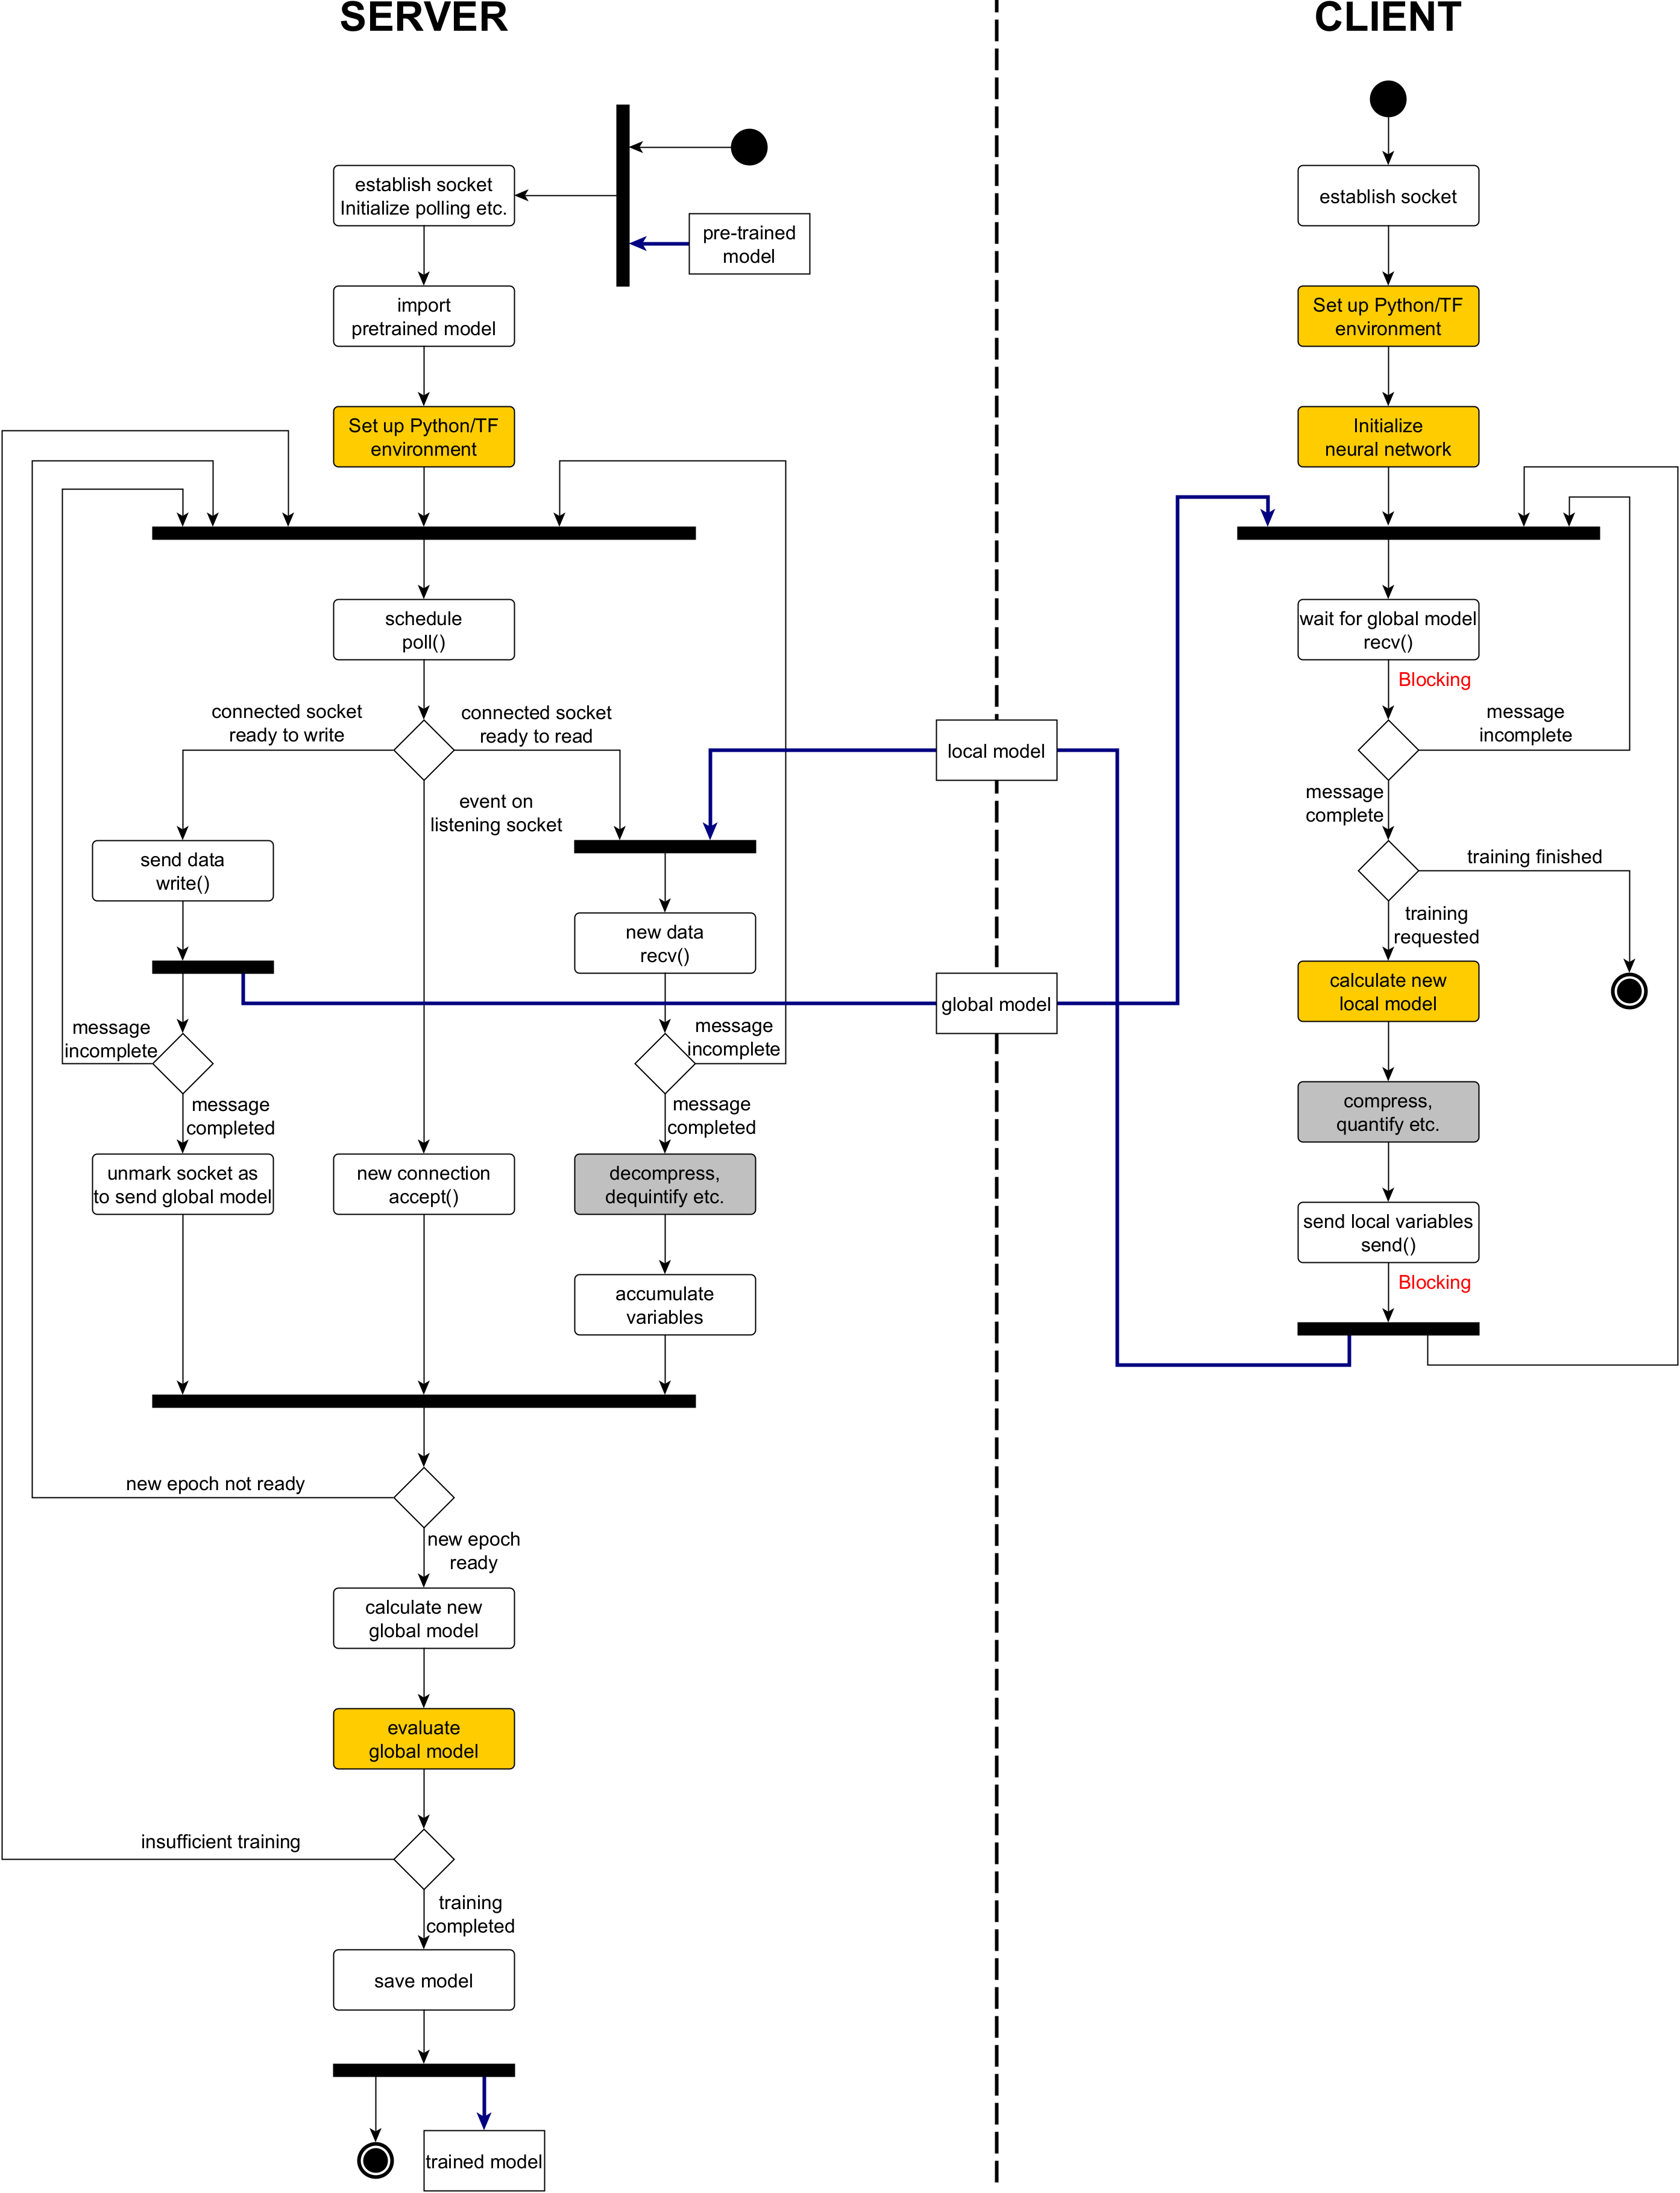
\includegraphics[ width=\textwidth, height=\textheight, keepaspectratio]{Images/block_diagrams/top.png}
        \decoRule
        \caption[Server - Client Activity Diagram]{Server - Client Activity Diagram: Yellow states are modelled with TensorFlow, while grey states are not essential for FL. Blue arrows represent data movements. Error conditions and states are not displayed.}
        \label{fig:server_client_activity_diagram}
\end{figure}
% \subsection{Life cycle of a model?} figure 4.1

\subsection{Communication Scheme}
As stated in section \ref{sec:FL_architecture}, the server and the clients are separate processes that communicate over sockets. A concrete, predefined communication system is needed to accomplish this in a reliable manner. The server holds the barest amount of information on the clients, just what is necessary to stay in connection and communicate, to adhere to the cross-device FL setting.
As such, the server can not address clients directly and messages must be generic. Furthermore, each message must be independent from the rest and self sufficient. As a result, messages sent by the server to clients must be general and self-sufficient.

Algorithmic solutions can reduce communication, but communication must be kept to a minimum in systemic level too. The messages, to be as compact as possible, only include their model and a few bytes of metadata required by the FL algorithm. Furthermore, they are C-aligned arrays, which means there are no delimiters between their values, or hidden metadata from predefined protocols of higher abstraction, such as Protobuf.

Minimizing communication frequency is another strategy used for cutting down on communication time. Any message send by the server that contains the global model, can be interpreted as an request to train it. Furthermore, if a client sends its local model, it can be presumed that it completed its task. As a result, each epoch only these two messages are required, and any synchronization or confirmation messages are unnecessary. With this approach, it is necessary for every party to interpret the messages in a same predefined way.

\begin{table}[H]
    \center
    \begin{tabular}{ | c | }
        \hline
        Server to client message\\
        \hline\hline
        flags\\
        \hline
        GE\\
        \hline
        global model variables\\
        ...\\
        \hline
        \multicolumn{1}{ c }{ } \\
    \end{tabular}
    \quad
    \begin{tabular}{ | c | }
        \hline
        Client to server message\\
        \hline\hline
        GE\\
        \hline
        local loss\\
        \hline
        local accuracy\\
        \hline
        model variables / deltas\\
        ...\\
        \hline
    \end{tabular}
    \caption[Communication Scheme]{The format of the communication between the server and clients.}
    \label{table:FL messages structure}
\end{table}

The format of the messages is shown in Table \ref{table:FL messages structure}. The flags field is intended to communicate particular instructions to clients, such as the message is the final one and no more communication will be accepted or that the client should initialize the model. The GE field is used to discard stragglers, as the server can quickly reject any messages from an earlier GE. The local loss and accuracy fields are used to facilitate complex algorithms, such as ignoring local models with poor accuracy or higher loss than the prior GE. The global and local model parameters are the last part of the format and make up the bulk of the messages.

\subsection{Model Library}
Most ML models, if not all of them, are meant to be trainable in a federated environment. To demonstrate the accuracy of the developed FL environment, a library of ten typical models has been created. As the training problem is image recognition, the majority of the models are CNNs. However, models of different architectures, such as deep and residual ANNs, are also included.

\begin{enumerate}

    \item The simplest model in the library is a DNN architecture. It consists of three fully connected ReLU activated layers with 128, 1024 and 128 neurons respectively, followed by a Softmax layer. In total, it contains 365,066 weights for an approximate size of 1.46 MBytes.
    
    \item The first CNN model follows the original LeNet-5 architecture. It has two convolutional layers of 6 and 16 \(5\times5\) kernels, each one accompanied by an average pooling layer with \(2\times2\) pool size. They are followed by two fully connected layers of 120 and 84 neurons, and a Softmax layer. All layers, except the final one, are activated with the hyperbolic tangent function. In total, it contains 61,706 weights for an approximate size of 0.25 MBytes.
    
    \item For the following experiments, the model most used is a CNN architecture consisting of two convolutional ReLU activated layers of 32 and 64 \(3\times3\) kernels, each accompanied by a max pooling layer with \(2\times2\) pool size. They are followed a 128-neuron fully connected ReLU activated layer, and a Softmax layer. It contains 421,642 weights for an approximate size of 1.69 MBytes. This architecture is compact enough to enable rapid experimentation and testing while being sufficiently sophisticated to provide an acceptable level of accuracy and necessitate several training epochs.
    
    \item The CNN used in the original FL work \cite{FL-original-paper} is also included in the model library. Its architecture is fairly similar with the previous one, but with larger \(5\times5\) kernels, and a fully connected layer of 512 neurons. In total, it contains 1,663,370 weights for an approximate size of 6.65 MBytes.
    
    \item The next model included in the library aims to evaluate the FL environment with more sophisticated layers and combinations between them. It employs six convolutional layers, applies batch normalization on their outputs, and uses max pooling every two convolutions. There are 803,240 weights in it, giving it an approximate size of 3.2 MBytes.
    
    \item To test the FL environment with extremely large models, the AlexNet architecture have been implemented. The model consists of 46,764,746 weights for a message size of 187 MBytes. As a result, it is unfeasible to train it repeatedly, as the FL operation needs, with the current available resources. Instead, it was trained for a single epoch with a few training data and conservative hyperparameters, just to demonstrate that the FL environment has no model size constraints.

    \item For similar reasons the OverFeat-AlexNet architecture is included. This model is the largest one in the library, with 56,906,954 weights and a total size of 227 MBytes. The same constrains apllies.
    
    \item The inception module detailed in section \ref{Inception Module} is the foundation for two of the included models. The first one comprises of two such modules of different sizes and a Softmax layer. It has a total of 4,275,914 parameters and is about 17.1 MBytes in size.
    
    \item The second inception architecture includes a module sandwiched between two convolutional layers, and max pools the outputs of all three. The output of the module is also subjected to the dropout transformation. Furthermore, they are followed by two fully connected layers and then a Softmax layer. In total, there are 277,082 weights for a size of 1.1 MBytes.
    
    \item The final model is based on the residual architecture. It is consisted of two convolutional layers and a Softmax layers. The input of the network feeds the convolutional layers, but it also skips them and is directly connected to the Softmax layer. Furthermore, the dropout transformation is applied to the input of the Softmax layer. It has 539,466 parameters and is about 2.16 MBytes in size.
\end{enumerate}
